\documentclass{standalone}
\usepackage{tikz}
\begin{document}
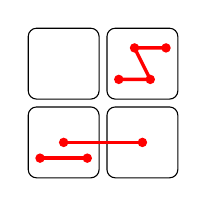
\begin{tikzpicture}[scale=1]
  % draw rounded cell boxes
  \draw[rounded corners=3pt] (0.05,0.05) rectangle (0.95,0.95);
  \draw[rounded corners=3pt] (0.05,1.05) rectangle (0.95,1.95);
  \draw[rounded corners=3pt] (1.05,0.05) rectangle (1.95,0.95);
  \draw[rounded corners=3pt] (1.05,1.05) rectangle (1.95,1.95);
  \fill[red] (0.2,0.3) circle (0.06);
  \fill[red] (0.8,0.3) circle (0.06);
  \draw[red, line width=1.2pt] (0.2,0.3) -- (0.8,0.3);
  \fill[red] (0.5,0.5) circle (0.06);
  \fill[red] (1.5,0.5) circle (0.06);
  \draw[red, line width=1.2pt] (0.5,0.5) -- (1.5,0.5);
  \fill[red] (1.2,1.3) circle (0.06);
  \fill[red] (1.4,1.7) circle (0.06);
  \fill[red] (1.6,1.3) circle (0.06);
  \fill[red] (1.8,1.7) circle (0.06);
  \draw[red, line width=1.2pt] (1.2,1.3) -- (1.6,1.3) -- (1.4,1.7) -- (1.8,1.7);
\end{tikzpicture}
\end{document}